\documentclass{article}
\usepackage{latexsym}
\usepackage{amsmath}
\usepackage[a4paper]{geometry}
\usepackage{fullpage}
\usepackage{hyperref}
\usepackage{booktabs}
\usepackage{graphicx}
\usepackage{tikz}
\usepackage{xcolor}
\usepackage[export]{adjustbox}
\usepackage{comment}
\usepackage{subcaption}
\usepackage[style=iso]{datetime2}
\usepackage{cleveref}
\usepackage{listings}

%\usetikzlibrary{calc}
\usetikzlibrary{arrows,positioning} 
\tikzset{
    %Define style for course boxes
    courseboxv/.style={
           rectangle,
           draw=blue!50!black, very thick,
           fill=blue!10,
           minimum height=8cm,
           minimum width=4cm,
           text width=3.9cm,
           text centered,
           font=\bfseries\sffamily},
    courseboxh/.style={
           courseboxv,
           minimum height=4cm,
           minimum width=8cm,
           text width=7.9cm},
    courseboxhh/.style={
           courseboxh,
           minimum height=4cm,
           minimum width=16cm,
           text width=15.9cm}
}
\def\frameseparation{1.5cm}
\def\scalingfactor{.8}

\newcommand{\secref}[1]{Section~\ref{sec:#1}}
\newcommand{\secreff}[2]{Sections \ref{sec:#1} and \ref{sec:#2}}
\newcommand{\eqnref}[1]{Equation~\eqref{eq:#1}}
\newcommand{\eqnreff}[2]{Equations \eqref{eq:#1} and \eqref{eq:#2}}
\newcommand{\eqnrefff}[3]{Equations \eqref{eq:#1}, \eqref{eq:#2} and \eqref{eq:#3}}
\newcommand{\figref}[1]{Figure \ref{fig:#1}} 
\newcommand{\figreff}[2]{Figures \ref{fig:#1} and \ref{fig:#2}}
\newcommand{\figrefff}[3]{Figures \ref{fig:#1}, \ref{fig:#2} and \ref{fig:#3}}
\newcommand{\tabref}[1]{Table~\ref{tab:#1}}
\newcommand{\tabreff}[2]{Tables~\ref{tab:#1} and \ref{tab:#2}}
\newcommand{\tabrefff}[3]{Tables~\ref{tab:#1}, \ref{tab:#2} and \ref{tab:#3}}

\def\year{2024--2025}
\title{EITA65 Design of Systems for Digital Transformation\\\year}
%\title{EITA65 Digitalisering -- realisering och systemdesign med användarperspektiv\\\year}
\author{\huge Interaction with Drones\\\textbf{Optional} Drone Project -- Part 6}
%\\Version \DTMnow}
%\date{}

\begin{document}
\newgeometry{left=2.5cm,right=2.5cm,bottom=1.5cm}% for placing course schematic lower on first page
\clearpage\maketitle
\thispagestyle{empty}% to remove page numbering on first page

\begin{itemize}
\item In this project, you will work together in groups  of 3 or 4.  
\item You will not get detailed step-by-step instructions. Figuring out how to reach the goal is part of the project. (being a collaborative doer)
\item The results of this project part will be used in the next, so document your work.
\end{itemize}

\vspace{.1cm}
\begin{center}
\begin{tabular}{l}
\toprule[1.5pt]
\parbox{0.8\linewidth}{
\vspace{.2cm}{\Large Learning goals:}
\begin{itemize}
    \item Practice integration with Raspberry Pi using Sense Hat.
    \item Design a human-drone interaction flow using LED matrix and joystick on Sense Hat, as well as an external speaker. 
    \item Implement your interaction flow in Python and integrate it to your drone simulation.
    \item Practice active collaboration with your group members.
\end{itemize}}\\
\bottomrule[1.5pt]
\end{tabular}
\end{center}



\vfill
% \begin{center}
% \includegraphics[width=120mm]{rpi4_no_bg.png}
% \end{center}
\begin{center}
\huge Good luck!
\end{center}
\vspace{2cm}


\begin{comment}
\begin{center}
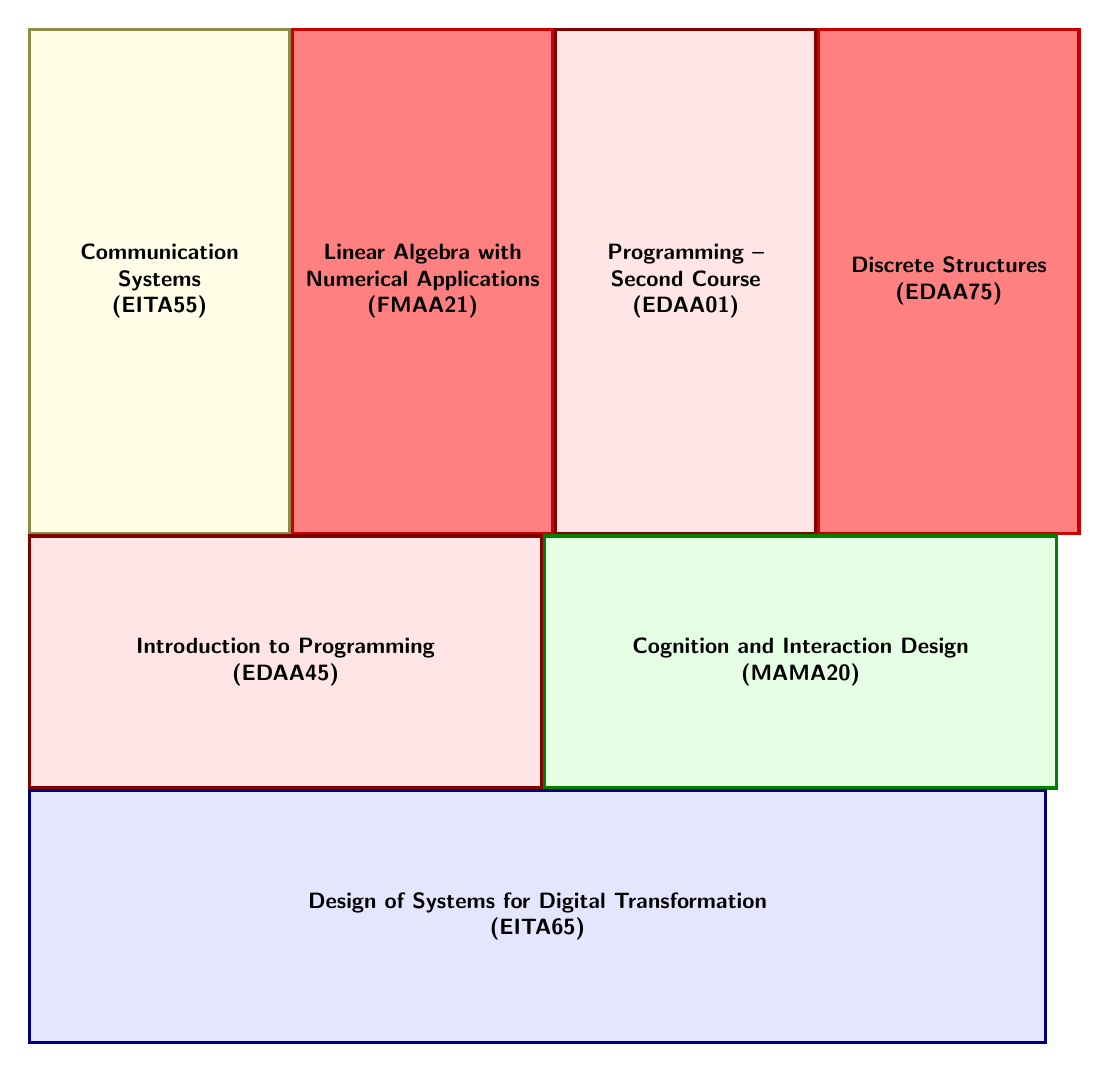
\begin{tikzpicture}[>=latex, node distance=0cm,scale=\scalingfactor,every node/.style={scale=\scalingfactor}]
\node[courseboxv, draw=yellow!50!black, fill=yellow!10] (EITA55) {Communication Systems\\(EITA55)};
\node[courseboxv, draw=red!80!black, fill=red!50, anchor=west] (FMAA21) at (EITA55.east){Linear Algebra with Numerical Applications\\(FMAA21)};
\node[courseboxv, draw=red!50!black, fill=red!10, anchor=west] (EDAA01) at (FMAA21.east){Programming -- Second Course\\(EDAA01)};
\node[courseboxv, draw=red!80!black, fill=red!50, anchor=west] (EDAA75) at (EDAA01.east){Discrete Structures\\(EDAA75)};
%\node[courseboxh, preaction={clip, postaction={fill=red!10, draw=red!50!black, line width=2mm}}, anchor=north west] (EDAA45) at (EITA55.south west){Introduction to Programming\\(EDAA45)};
\node[courseboxh, draw=red!50!black, fill=red!10, anchor=north west] (EDAA45) at (EITA55.south west){Introduction to Programming\\(EDAA45)};
%\node[courseboxh, draw=green!50!black, fill=green!10, anchor=west] (MAMA20) at (EDAA45.east){Cognition and Interaction Design\\(MAMA20)};
\node[courseboxh, draw=green!50!black, fill=green!10, right=of EDAA45] (MAMA20) {Cognition and Interaction Design\\(MAMA20)};
\node[courseboxhh, anchor=north west] (EITA65) at (EDAA45.south west){Design of Systems for Digital Transformation\\(EITA65)};
%\node[anchor=south east, inner sep=2pt, font=\bfseries\sffamily\scriptsize] at (EDA625.south east) {Helsingborg};
%\path[->,draw=black,dotted,thick] (EIT060.east) -- (EITF05.west);
%\path[->,draw=black,dotted,thick] (EIT060.south) -- (EITN50.north);
%\path[->,draw=black,dotted,thick] (EITF05.south) -- (EITN41.north);
%\draw[draw=blue!50!black, very thick] ($(EIT060.north west)+(-\frameseparation,\frameseparation)$) rectangle ($(EDA625.south east)+(\frameseparation,-\frameseparation)$);
\end{tikzpicture}
\end{center}
\end{comment}



\restoregeometry

\newpage


\section{Introduction}
In the last part of LP3 project, you will need to design a human-drone interaction flow for your drone package delivery system. In the flow, your drone Pi will need to react to every status change using both the LED matrix on its Sense HAT and an external speaker. The joystick will also be used to interact with the drone, simulating human actions such as handing over and signing for a package.

Something you need to prepare before the lab:
\begin{enumerate}
    \item You still work as a group of 3 or 4. 
    \item Make sure your Sense HAT is mounted on your Raspberry Pi and that it works without any problem. Only Drone Pis will need Sense HATs. If you find that your Sense HAT is broken, coordinate with your group members or let us know if there are not enough Sense HATs in your group.
    \item You are encouraged to bring your own speakers/audio devices. Both wired speaker or Bluetooth speaker work. It is preferred that each Drone Pi has an attached audio device, but it also works if there is only one in the group. The TAs will bring some for you to borrow during lab sessions, but they may not have enough to equip all groups fully. You can connect a Bluetooth speaker to your Pi by the same way as you do with your other devices. Follow pairing instructions of your Bluetooth speaker. In your Pi click on Bluetooth icon, "Make Discoverable" and "Add Device".
    You can also follow \textcolor{blue}{\href{https://raspberrydiy.com/connect-raspberry-pi-bluetooth-speaker/}{this instruction}}, if you encounter issues to connect the Bluetooth speaker to your Pi.  
\end{enumerate}

In this part you will modify your code from the previous lab (part 2). It might be a good idea to
begin by making a backup copy of your entire solution to part 2 before you begin working on this lab. (files in \verb!/pi!). No changes are needed in \verb!/webserver!, but you will need to replace your \verb!index.html! file with the one provided in \textcolor{blue}{\href{https://github.com/HaoruiPeng/InfoCom-LP3-Lab3}{this GitHub repository}}. The new HTML has three color options representing the different statuses of a drone:
\begin{itemize}
    \item \textbf{idle}
    \begin{itemize}
        \item Displayed in green.
        \item Drone can take a delivery order.
    \end{itemize}
    \item \textbf{busy}
    \begin{itemize}
        \item Displayed in red.
        \item Drone in mission, moving.
    \end{itemize}
    
    \item \textbf{waiting}
    \begin{itemize}
        \item Displayed in yellow.
        \item Drone in mission,  waiting for human confirmation for loading a package or signing for a package.
    \end{itemize}
\end{itemize}
The interaction flow will be mostly implemented in the \verb!/pi/simulator.py! file. You can use your own script from part 2, or use the template provided in the GitHub repository, which is the same as the template in part 2, but a bit cleaner.

As mentioned before, you will need a speaker to play some sound effects on the drone to indicate a status switch. In this lab we use the \verb!pygame! package to play music or sound effects in Python. Please read the instruction in \verb!/pygame-music! in the repository for installing and using the package.


\section{Interaction Flow}
In this part, you will need to design an interaction flow. In the simulation we used in part two, the drone is not interactive. It can only display two different statuses, and it follows a simplified action flow to simulate the processes of package delivery, with two addresses sent by the route planner on the server Pi. The action flow in part 2 is depicted in \Cref{fig:old}.

In the new flow you design, you will need to add human interaction with the drone, and the drone can display different symbols and make some sound effects indicating different status. The new flow should at least include the states and interactions as shown in \Cref{fig:new}. You are welcome to design your own flow based on the example in \Cref{fig:new}.

% An example of the finished task is given \textcolor{blue}{\href{https://lunduniversityo365-my.sharepoint.com/:v:/g/personal/ha8653pe_lu_se/EQTekEQwRQhNknu-U8_7LYIBUcTzMELS32saOETIbiWEUg?e=pU2Tsb}{in this video}}. In the video, the printouts on the terminal are from the drone, indicating state switches in the simulation. There are three symbols displayed on the LED matrix:
%\begin{itemize}
%     \item Green alien: idle status.
%     \item Red flashing creeper: moving, busy status. 
 %    \item Steady Steve (with a bell sound): waiting for loading/signing for package (realized by pressing on the joystick).
% \end{itemize}
    The LED matrix should indicate the current state in the workflow for the drone and pressing the joystick simulates confirming loading/signing for the package. Sound clips are uploaded to the repository. You could do this lab with the provided sound clips, but now might also be a good opportunity to start experimenting with interaction sounds on your own. There are lots and lots of sound files to search for and download online: \textcolor{blue}{\href{www.freesound.org}{Freesound}} is a great starting point or just Internet-search “sound fx”. However, when you find sound files online, they may be too long or have compound sounds. Or there could be an annoying pause in the recording before the actual sound, which negatively affects the possibility to use it as a well-timed button sound in your interface. So, you might end up wanting to trim beginnings and ends of sound files, or even filter them. You can do this on your Pi, using \textcolor{blue}{\href{https://www.audacityteam.org/}{Audacity}}, which can be installed with command \verb!sudo apt-get install audacity!. You could also install and use it on your regular computer, but then you’ll have to move the sound files to the Pi later. If you are new to audio editing, start with the guide \textcolor{blue}{\href{https://userguiding.com/blog/audacity-tutorial/}{“Getting started with Audacity”}}. A handy list of tips can be found in the video \textcolor{blue}{\href{https://www.youtube.com/watch?v=WWFvG1-AmNk}{“Audacity Editing for beginners, 16 tips in 9 minutes”}}. 
 
\begin{figure}[h]
    \centering
    \includegraphics[width=0.4\linewidth]{old.png}
    \caption{Action flow of previous simulation}
    \label{fig:old}
\end{figure}

\begin{figure}[h]
    \centering
    \includegraphics[width=0.8\linewidth]{new.png}
    \caption{Minimum requirements of new interaction flow}
    \label{fig:new}
\end{figure}


% \begin{thebibliography}{10}
% \bibliographystyle{plain}

% \bibitem{json} JavaScript Object Notation (JSON) -- Wikipedia, \url{https://en.wikipedia.org/wiki/JSON}, last accessed on 2022-01-20.

% \bibitem{OSM} OpenStreetMap, \url{https://www.openstreetmap.org/#map=14/55.7059/13.2005}, last accessed on 2022-01-20.

% \bibitem{deco} Python decorator, \url{https://python-3-patterns-idioms-test.readthedocs.io/en/latest/PythonDecorators.html}, last accessed on 2022-01-20.

% \end{thebibliography}

\end{document}
